\chapter{Passband Filter}
\section{Setup}
The device, showed in figure \ref{passband},  has two ports which have been
connected to the VNA ports. On the VNA software we set the frequency range to 
be initially between 10MHz and 6.5GHz for the analysis. Then, by looking at the device's 
response, we focused on the range 1.5GHz-3GHz, which is the one worth to be analyzed. The results have been extracted
as Touchstone files and then they have been elaborated using python, in particular using the \texttt{scikit-rf} module.
\begin{figure}[H]
    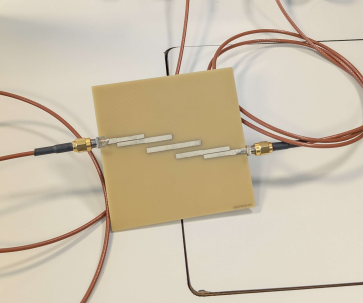
\includegraphics[width=0.5\textwidth]{leopart/passband.png}
    \centering
    \caption{Image of the device connected to the VNA}
    \label{passband}
\end{figure}

\section{Analysis of the measurements}
By looking at figure \ref{plots_full}, which shows the magnitude of the signal of the respective channel, is it clear that the device has a reciprocal response
between the two ports, since the plots of $S11$,$S22$ are identical as well as $S12$,$S21$ plots. So, for the rest of the analysis,
we will focus only on the $S22$ and $S12$ parameters.
\begin{figure}[H]
    \centering
    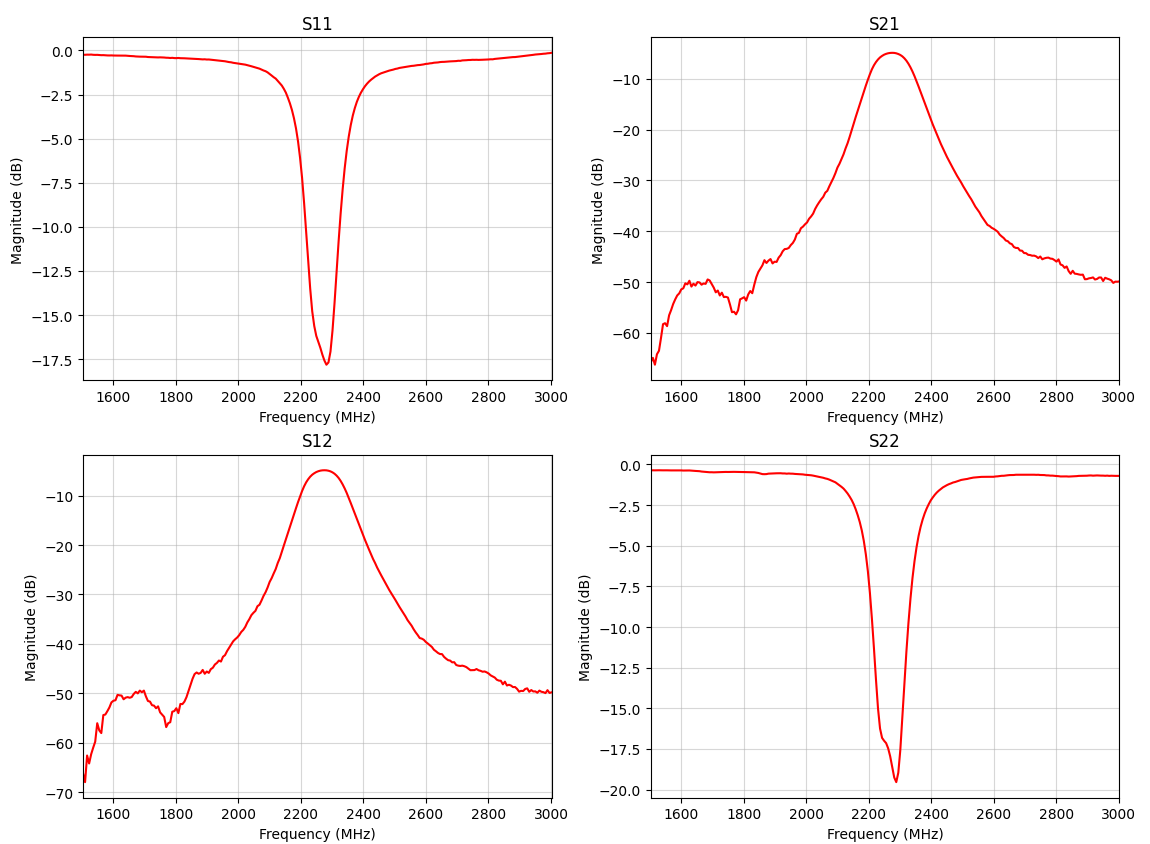
\includegraphics[width=0.8\textwidth]{leopart/plot_full.png}
    \caption{Plots of the parameters of the Scattering matrix}
    \label{plots_full}
\end{figure}
The analysis of the $S22$ and $S12$ parameters is summarized in table \ref{tab_pb}.
\begin{table}[h]
    \centering
    \label{tab_pb}
    \begin{tabular}{|l|c|c|c|}
        \hline
        \textbf{Parameter} & \textbf{Peak frequency [MHz]} & \textbf{Magnitude on peak [dB]} & \textbf{Bandwidth [MHz]} \\
        \hline
        $S_{22}$ & 2287 & -19.53 & 64.90 \\
        \hline
        $S_{12}$ & 2275 & -4.88 & 123.31 \\
        \hline
    \end{tabular}
    \caption{Analysis of the $S22$ and $S12$ parameters}
\end{table}
By examinating the $S12$ plot, we understand that the device is allowing the signal to pass through it in a frequency range around $2275$MHz 

me so rotto er cazzo

\section{Summary}
here i just summarize the findings that i just explained in the rpevious section
\chapter{Antenna}
\section{Setup}
\section{Analysis of the measurements}
\section{Summary}